\label{ch:proced}
After describing different approaches to compute PESs in chapter \ref{ch:calcPES} and pointing out why the DO formalism combined with a finite element method for the computation of the photoelectron function is well-suited for our needs, in this chapter the protocol as being used to obtain the PESs is be presented.

In the first section the computation of the wave functions of initial (unionised) and final (ionised) states as well as the genaral procedure used to compute the DOs is described.
Thereafter, in section \ref{sec:grid} the setup of the finite element system that is used to compute the free electron function as well as the dipole matrix element are explained which is implemented in the program \prog{FreeWilly} \cite{FreeWilly} in the framework of this thesis.

\section{Bound State Functions}
The DO formalism as it is described in \ref{ch:do} can be used with any self-consistent field method which can predict excited state energies and wave functions.
In this work,  density functional theory (DFT) is used for ground state calculations and its time dependent counterpart TDDFT to compute excited state energies.
The DFT formalism which is introduced in the sections \ref{ch:dft} and \ref{ch:tddft} has shown to be accurate and numerically cheap.
%In this work the calculations are done using a locally modified version of the program package \prog{NWChem} \cite{nwchem} where a more verbose output enables the reconstruction of all molecular orbitals and thus the computation of the DOs.

\subsection{Ground State Density}
\label{ch:dft}
The DFT is formally based on the Hohenberg-Kohn theorems \cite{HohenbergKohn} which state that the ground-state electron density determines the potential in the SE and with this also the wave-function.
Moreover, the second Hohenberg-Kohn theorem states that the energy of the ground state can be found variationally from the density.
Thus, the electron density contains all information needed and the computation of the $N$-electron wave function can be omitted.
Since the Hohenberg-Kohn theorems do not point out a way how to determine the electron density without knowing the wave-function, usually the Kohn-Sham scheme \cite{KohnSham} is used where the electrons are described as non-interacting particles in a respective pseudo-potential that is constructed such that the electron density of these Kohn-Sham orbitals corresponds to the real electron density.
Since the particles do not interact with each other, the Kohn-Sham orbitals $\Psi_j(\vec{r})$ can be obtaind from the one-particle SE
\begin{equation}
\left( -\frac 12  \nabla^2 + V_\text{eff}(\vec{r}) \right) \Psi_j(\vec{r})=\epsilon_j \Psi_j(\vec{r})
\end{equation}
where $\epsilon_j$ is the binding energy of the respective Kohn-Sham orbital and the effective potential 
\begin{equation}
V_\text{eff}(\vec{r})=V_\text{ext}(\vec{r})+ \int \frac{\rho(\vec{r}')}{|\vec{r}-\vec{r}'|} d\vec{r}' + V_\text{xc}(\vec{r})
\end{equation}
can be separated into the external potential $V_\text{ext}(\vec{r})$, which consists of the attractive nuclear ESP and external fields, the electrostatic interaction of the particles where $\rho(\vec{r})=\sum_{i\neq j} |\Psi_i|^2$ and the exchange-correlation potential $V_\text{xc}(\vec{r})$ which contains the complexity of the electronic interaction \cite{baerRSH}.
The exchange correlation potential $V_\text{xc}(\vec{r})$ contains, besides contributions from exchange and correlation, also the error of kinetic energy in the Kohn-Sham scheme to account for the fact that the Kohn-Sham wave-functions differ from the real orbitals and thus have another kinetic energy as well \cite{Holthausen}.

Assuming that the Kohn-Sham orbitals coincide with the physical orbitals, the exchange potential acts on an orbital $\Psi_i(\vec{r})$ as
\begin{equation} \label{eq:HF_exch}
V_{x;j}(\vec{r})\Psi_i(\vec{r}) =\int \frac{\Psi_j^\dagger(\vec{r}') \Psi_i(\vec{r}')}{\left|\vec{r}-\vec{r'}\right|} d\vec{r}' \Psi_j(\vec{r})
\end{equation}
and thus is non-local \cite{Holthausen}. % the ``exact'' exchange energy thus corresponds the term $E_{x}=\sum_{i<j}\int \Psi_i^\dagger(\vec{r}) V_{x;j}(\vec{r}) \Psi_i(\vec{r}) d\vec{r}$  respectively.
In DFT usually the exchange energy is approximated as a local functional of the density and its derivative, leading to the so-called local density approximation and gradient corrected functionals \cite{baerRSH}.
The Becke \cite{blyp} exchange-functional used in this work has the form
\begin{equation} \label{eq:blypXC}
E_x=\frac 32 \left(\frac{3}{4\pi}\right)^\frac 13 \sum_\sigma \int \rho_\sigma(\vec{r})^\frac 43 d^3\vec{r} 
-\beta \sum_\sigma \int \rho(\vec{r})^\frac 43 \frac{x_\sigma(\vec{r})^2}{1+6\beta x_\sigma \text{sinh}^{-1}( x_\sigma (\vec{r}))} d^3\vec{r}
\end{equation}
where the first summand corresponds to the local density approximation and the second is a semi-empirical gradient correction, $\sigma$ denotes the spin polarisations and $x_\sigma(\vec{r})=\frac{|\nabla \rho_\sigma(\vec{r})|}{\rho_\sigma^\frac 43}$. 
The gradient correction in this functional is constructed such that the asymptotic behaviour of the exchange energy and electron density follow
\begin{align}
  \lim_{r\rightarrow\infty} E_x^\sigma(\vec{r}) & =-\frac{1}{|\vec{r}|} \\
  \lim_{r\rightarrow\infty} \rho(\vec{r}) & =e^{-a_\sigma |\vec{r}|}
\end{align}
with $a_\sigma$ is a constant related to the ionisation potential of the system under study \cite{blyp}.
The prefactor of the gradient correction, $\beta$, was determined by fitting to several atomic noble-gas systems and is set to be $\beta=0.0042$ in atomic units \cite{blyp}.

%Finally, the correlation energy is defined as the difference between the sum of the previously discussed terms and the correct energy.
The correlation potential finally is defined as the functional derivative of the correlation energy with respect to the electron density $V_c(\vec{r})=\frac{\partial E_c[\rho]}{\partial\rho(\vec{r})}$.
In the case of the
The LYP-correlation energy functional is based on the Colle-Salvetti formula which estimates the correlation energy in the Hartree-Fock approach and introduces two parameters that are set by fitting to experimental data \cite{lyp}.

\subsection{Properties of Excited States}
\label{ch:tddft}
The DFT is not only a well-established method to obtain ground-state properties of many different kinds of systems, but it has also a time-dependent counterpart, formally based on the Runge-Gro\ss\, theorem \cite{RungeGross}.
Commonly, when referring to TDDFT, respective the linear-response scheme is meant \cite{dreuw}.
It is a first order perturbation expansion and can be used to obtain the energies and occupation numbers of excited states using the so-called Casida-equation \cite{casida}
\begin{equation} \label{eq:casida}
\begin{bmatrix} \mat{A} & \mat{B} \\ \mat{B}^\dagger & \mat{A}^\dagger\end{bmatrix}
\begin{bmatrix} \vec{X} \\ \vec{Y} \end{bmatrix} =
\omega \begin{bmatrix} \mat{1} & \mat{0} \\ \mat{0} & -\mat{1}\end{bmatrix}
\begin{bmatrix} \vec{X} \\ \vec{Y} \end{bmatrix}
\end{equation}
where the matrix elements are
\begin{align}
\mat{A}_{ia,jb}& =\delta_{ij}\delta_{ab}(\varepsilon_a-\varepsilon_i)+ 
\int \int d\vec{r} d\vec{r}'\frac{ \Psi_i(\vec{r}) \Psi_a(\vec{r})  \Psi_j(\vec{r}') \Psi_b(\vec{r}')- 
\Psi_i(\vec{r}) \Psi_j(\vec{r}) \Psi_a(\vec{r}') \Psi_b(\vec{r}')}{|\vec{r}-\vec{r}'|} ,\\
\mat{B}_{ia,jb}& = \int \int d\vec{r} d\vec{r}'\frac{\Psi_i(\vec{r}) \Psi_a(\vec{r})  \Psi_b(\vec{r}') \Psi_j(\vec{r}')- 
\Psi_i(\vec{r}) \Psi_b(\vec{r})  \Psi_a(\vec{r}') \Psi_j(\vec{r}')}{|\vec{r}-\vec{r}'|}
\end{align}
where $i,j$ denote occupied and $a,b$ virtual states and $\mat{1}$ is the unity matrix, $\varepsilon_\alpha$ are (Kohn-Sham) orbital binding energies of the Kohn-Sham orbitals $\Psi_\alpha(\vec{r})$.
The indices $i,j$ and $a,b$ denote occupied and virtual orbitals with binding energy $\varepsilon_i, \varepsilon_a$ respectively \cite{dreuw}.
The Casida equation (\ref{eq:casida}) is an non-hermitian eigenvalue problem whose eigenvalues $\omega$ correspond to the transition energies and the eigenvectors denote the transition coefficients.
The different blocks in equation (\ref{eq:casida}) have different physical interpretation.
As the negative sign of the transition energy in the lower block indicates, lower half of the eigen vector, denoted as $\vec{Y}$, corresponds to negative excitation energies $\varepsilon_i$ and can be assigned to de-excitations from virtual orbitals which makes no physical sense if the reference state is a ground state \cite{dreuw}.
Since the matrix $\mat{B}$ contains usually only small elements, it is often set to zero which is refferred to as Tamm-Dancoff approximation and reduces the original equation to a hermitian equation of half dimensionality \cite{casida}.

\subsection{OTRSH-scheme}
%One main issue concerned with the DFT-formalism is that the approximate exchange functional decays exponentially instead of $\frac 1r$ and $\frac{1}{r^4}$ for the exchange and correlation terms respectively \cite{Bokareva}. \textcolor{red}{But the Becke functional should have fixed this!?}
One main issue concerned with the DFT-formalism is that the approximate exchange functional lead to wrong asymptotic behaviour of the electoron density.
The local density approximation leads to an exponential decay instead of $\frac 1r$ and $\frac{1}{r^4}$ for the exchange and correlation terms respectively \cite{Bokareva} which is improved significantly with gradient-corrected functionals but usually still yields spuirous behaviour \cite{baerRSH}.
This wrong behaviour affects the obtained wave functions and thus the orbital energies \cite{OT-RSH}.

To reduce this error, so-called range-separated hybrid (RSH) functionals are used, in which the DFT-exchange term as \textit{e.g.} the Becke functional (\ref{eq:blypXC}) is used for small interelectronic distances only, while at larger distances, where correlation effects are not that important, the Hartree-Fock exact-exchange (\ref{eq:HF_exch}) is used \cite{LC-tddft}.
The interchange between the schemes is done by the scheme
\begin{equation}
   \frac 1r = \underbrace{\frac{\alpha +\beta erf(\omega r)}{r}}_{\text{exact exchange}} +\underbrace{\frac{1-\alpha-\beta erf(\omega r)}{r}}_{\text{DFT exchange}}
\end{equation}
where $\alpha+\beta=1$ and $\omega$ are parameters to be chosen.
Besides taking the standard parameters that are fitted to a set of testing-systems, ab-initio schemes for chosing $\alpha$ and $\omega$ are available which are referred to as optimally-tuned RSH (OTRSH) schemes.
Using such a scheme, the degrees of freedom obtained are used to optimise a particular system-property such as Koopmans' theorem by minimising the functional \cite{Bokareva}
\begin{equation}\label{eq:J_ao}
   J(\alpha_\text{opt},\omega_\text{opt})=\text{min}_{\alpha, \omega} \left\{ |E_N(\alpha,\omega)-E_{N-1}(\alpha,\omega)-\varepsilon_\text{HOMO}| \right\}
\end{equation}
or a similar one which can also account for lower-lying orbitals or the electron affinities which should resemble the binding energies of the lowest unoccupied molecular orbital (LUMO).

Another quantity to optimise is the derivative discontinuity \cite{derdis,sanchez,Autschbach} that is based on the fact that the exchange-correlation energy should be a straight line when varying the number of electrons from $N$ to $N+1$.
The slope of that line corresponds to the binding energy of the respective electron and thus is discontinuous at integer numbers of electrons.
The approximate exchange correlation functionals, however, usually do not fulfill this condition but the parameters $\alpha$ and $\beta$ can be tuned such that only small deviations can be observed \cite{Bokareva}.

For this optimization procedure the Gaussian package \prog{G09} \cite{g09} is used with the 6-31G(d) \cite{6-31g,6-31gd} basis set and the functional LC-BLYP \cite{lcblyp}. 
The ground state DFT calculation, determination of geometries and the linear-response TDDFT calculations have been conducted with a locally modified version of \prog{NWChem} \cite{nwchem}, employing the basis set def2-tzvp \cite{def2tzvp} without symmetry restrictions.
The Kohn-Sham orbitals (obtained by ground state DFT) and CI-coefficients (obtained by linear-response TDDFT which yields the configuration interaction singles expansion for a number of excited states) as well as the atomic overlap matrix are interfaced to the in-house software \prog{DYSON} \cite{MAgg} that computes the DOs.
The integration of the transition dipole matrix elements in eq. (\ref{eq:sigma_do}) finally is performed using \prog{ezDyson} \cite{ezDyson}.

\subsection{Obtaining the Electrostatic Potential and Dyson orbitals}
%Considering a state as linear combination of CI-states is denoted as weak-coupling representation \cite{McCarthy}.
The ESP used in this work is obtained with a modified version of \prog{NWChem} \cite{nwchem} where the points, at which this potential should be computed can be set by the user.
Setting these points to the quadrature points of the integration scheme requires some extra effort but has the great advantage that no interpolation needs to be done internaly.
An interpolation of the data in \prog{FreeWilly} \cite{FreeWilly} would require an interpolation of scattered data for which several schemes such as radial basis function interpolation or inverse distance interpolation are available but both methods give, if the parameters are chosen not accurately, spurious oscillations between the quadrature points and thus do not result an a smooth ESP.

The second external quantity needed to compute the intensities is the DO that is computed in the framework of this thesis with the in-house code \prog{DYSON} \cite{MAgg}.
To obtain the required data for this, the \prog{NWChem}-code is modified to produce more verbose output and the respective data are extracted and reformatted with a self-written script \cite{nwc2dy}.

\section{Free electron function}
The FEF is computed with a finite element scheme, using the program \prog{FreeWilly} \cite{FreeWilly} developed in the framework of this thesis.
It is based on the library \prog{Libmesh} \cite{libmesh} which itself uses several libraries for the required linear algebra and the mesh-setup.

\subsection{Setup of the Grid}
\label{sec:grid}
The most crucial part in a FEM simulation is the mesh being used. 
In the program \prog{FreeWilly} the distribution of elements is obtained from a set of points via Delaunay triangulation (see \ref{app:delaunay} for details) using the library \prog{tetgen} \cite{tetgen}.
The distribution of these points is responsible for the quality of the obtained solution via many parameters in a non-trivial way.
It is expected that the main parameters, the mesh should depend on are
\begin{description}
   \item[The molecular geometry] Close to the cores it should be denser, at larger distances a coarser grid is possible.
   \item[The kinetic energy] of the photo electron which gives the maximum distance between two points
   \item[The largest angular momentum of the Dyson orbital] determines the angular momentum of the photoelectron to be resembled.
\end{description}

In this work the generation of the point-distribution is chosen similarly to the grid used by Son and Chu \cite{Son_Chu} which is based on spherical distributions around the atoms whose overlapping regions are cut off.
To yield a reasonable mesh, the radii of these spheres need to be much larger than the bond lengths to avoid holes or interatomic gaps in the molecule, \textit{e.g.} between different ligands.
Using such a scheme, the parameters are determined by the size of the largest sphere $r_\text{max}$, number $N$ of spheres being used as well as the radial distribution and angular distributions, respectively.

For the radial distribution of $N$ spheres Son and Chu \cite{Son_Chu0} suggested the scheme
\begin{equation} \label{eq:son_map}
r_i=\frac{il}{N-i+\frac{lN}{r_\text{max}}} \qquad i=1,\hdots ,N 
\end{equation}
where $l$ is a free parameter.
Using this function, the smallest spheres ($i<<N$) are scaled linearly with distances $r_\text{max}/N$ whereas the distance of the largest spheres depends non-trivially on the parameters but can become very large.

To obtain better control of the distance between the inner spheres and the maximum distance which needs to be consiberably smaller than the wave length, in this work the formula
\begin{equation} \label{eq:tm_map}
r_i=\frac{il}{\left( \frac Ni \right)^p \left(\frac{Nl}{r_\text{max}}-1\right) +1} \qquad i=1,\hdots ,N 
\end{equation}
is suggested where two degrees of freedom $l$ and $p\geq 1$ are given and the condition $N<\frac{r_\text{max}}{l}$ needs to be fulfilled to prevent the singularity.
Here $l$ is an asymtotic expression for the distance between two spheres and the distance of inner spheres grows with the power $p+1$ so that it can be tuned freely.
%Thereby it is important to mention that in this scheme (in contrast to the above one) the (asymptotic for $r\rightarrow \infty$) maximum distance between two spheres is $l$ and hence could be physically chosen to $l\approx \frac \lambda 2$.

While the distribution of spheres follows, at least on a qualitative level, a clear scheme since it should always resemble the local kinetic energy, the distribution of points on the surface of each sphere more complicated.
Here, a regular distribution is a good choise, but on the non-linear topology of the sphere, regularity is in general more challenging.
While so-called geodesic grids are popular in earth sciences \cite{geodesic1,geodesic2,geodes_charge}, their construction allows only for exponentially growing mesh-sizes.
Another common approach is to use quadrature points of integration rules of a given order which lead to Lebedev-grids \cite{lebedev,lebedev2} and spherical t-designs \cite{t-design1, t-design2} that are found more often in quantum chemical contexts \cite{LebQC1,LebQC2,lebDFT,lebDFT2} and will be used in this thesis.
Further methods involve the search of extrem such as minimisation of the Riesz s-energy, and other geometric properties \cite{fliegeMaier,womersley,wom2,wom3} or a set of qualitatively lower but computationally much easier schemes such as the spherical fibonacci mapping \cite{fibonacci,fibonacci2}.
\begin{figure}
   %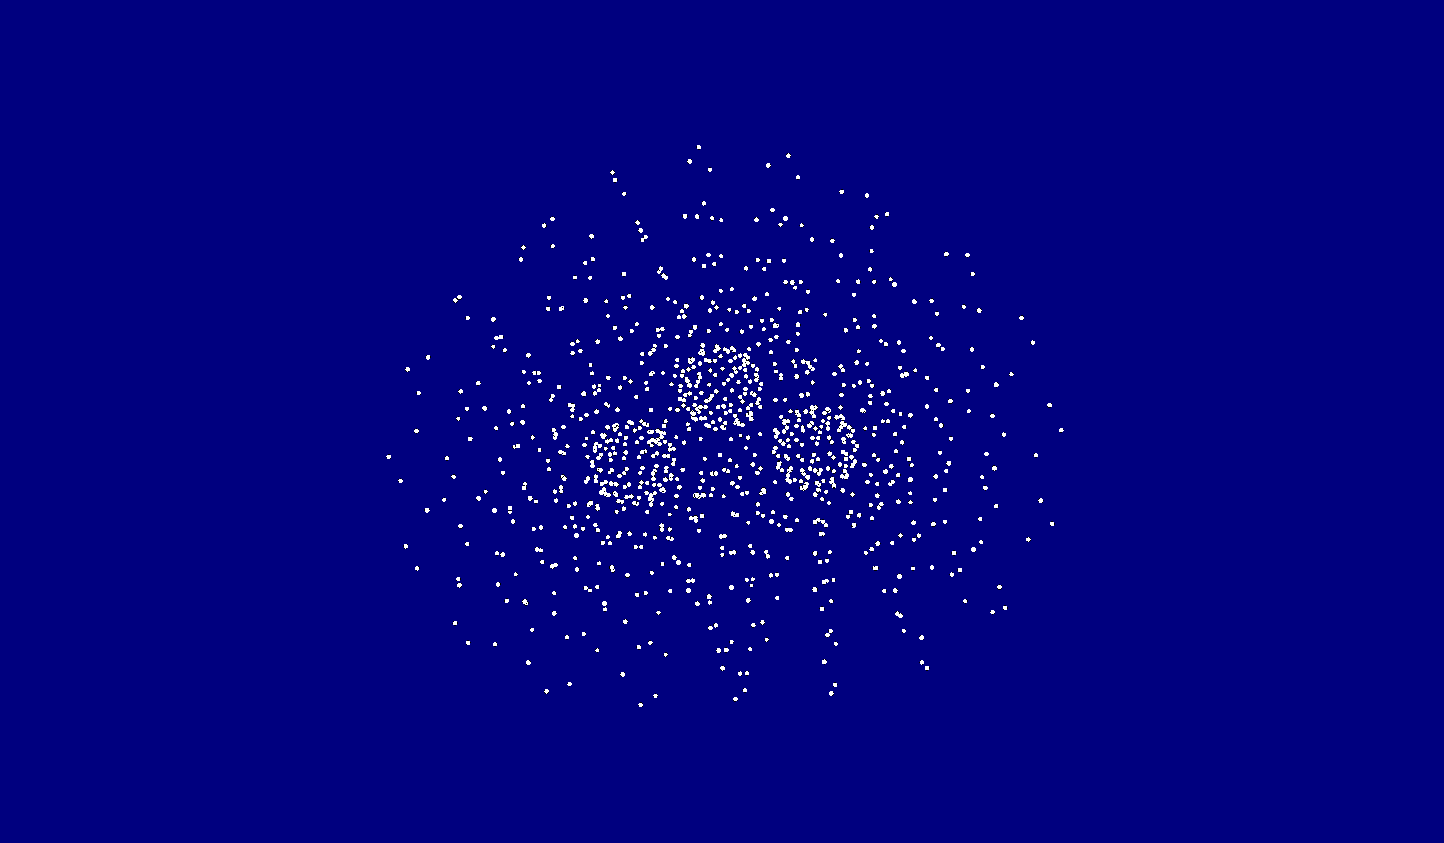
\includegraphics[width=0.5\textwidth]{water1}
   %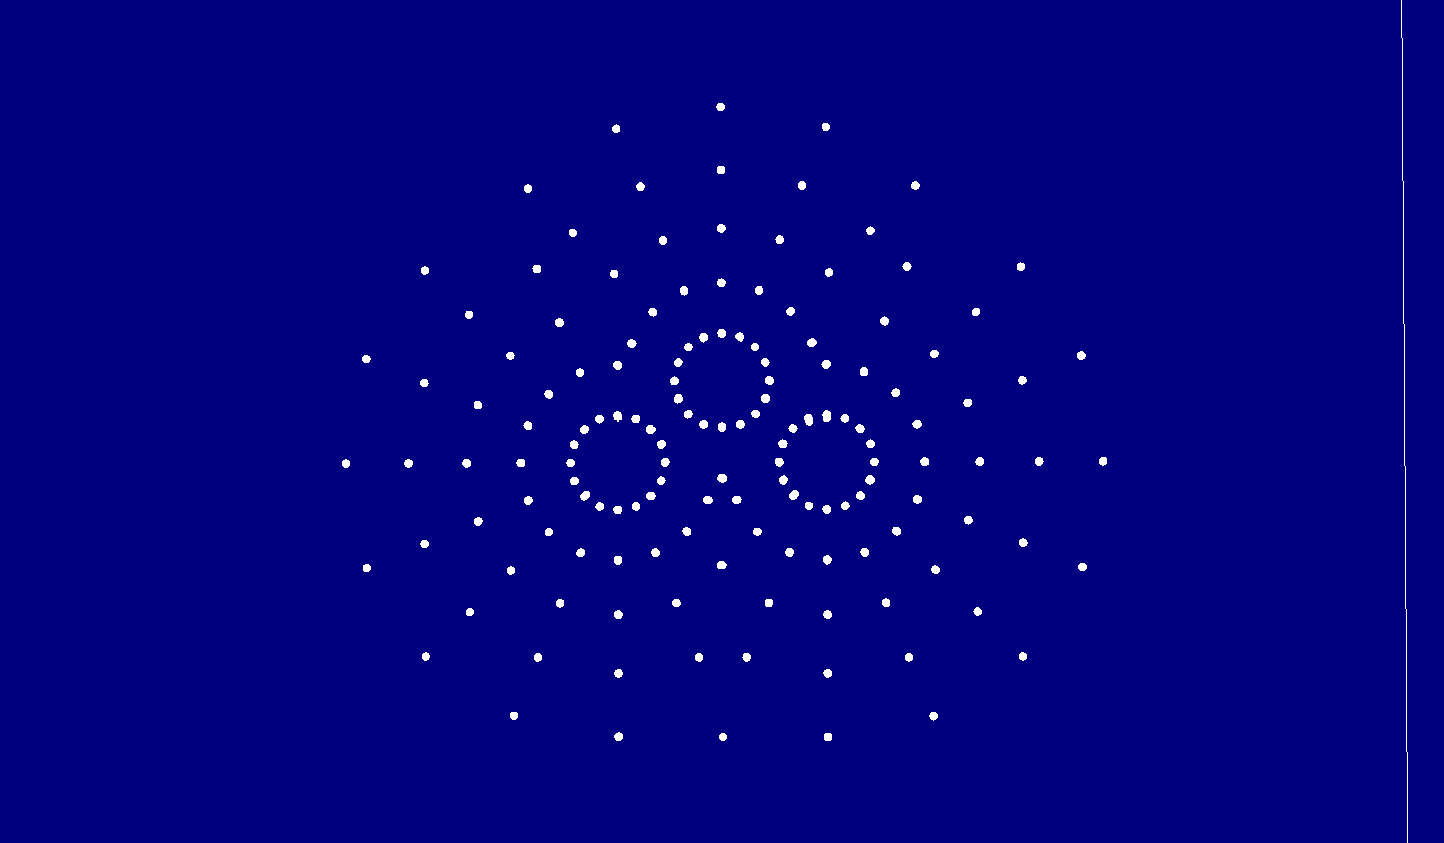
\includegraphics[width=0.5\textwidth]{water2}
   %\caption{Example of a mesh for the water-geometry. It consists of $5$ spheres with constant number of points per sphere. The overlapping regions are cut off. Left: cut through the nuclear plane. 
   %\textcolor{red}{add figure with distribution: tm}}
   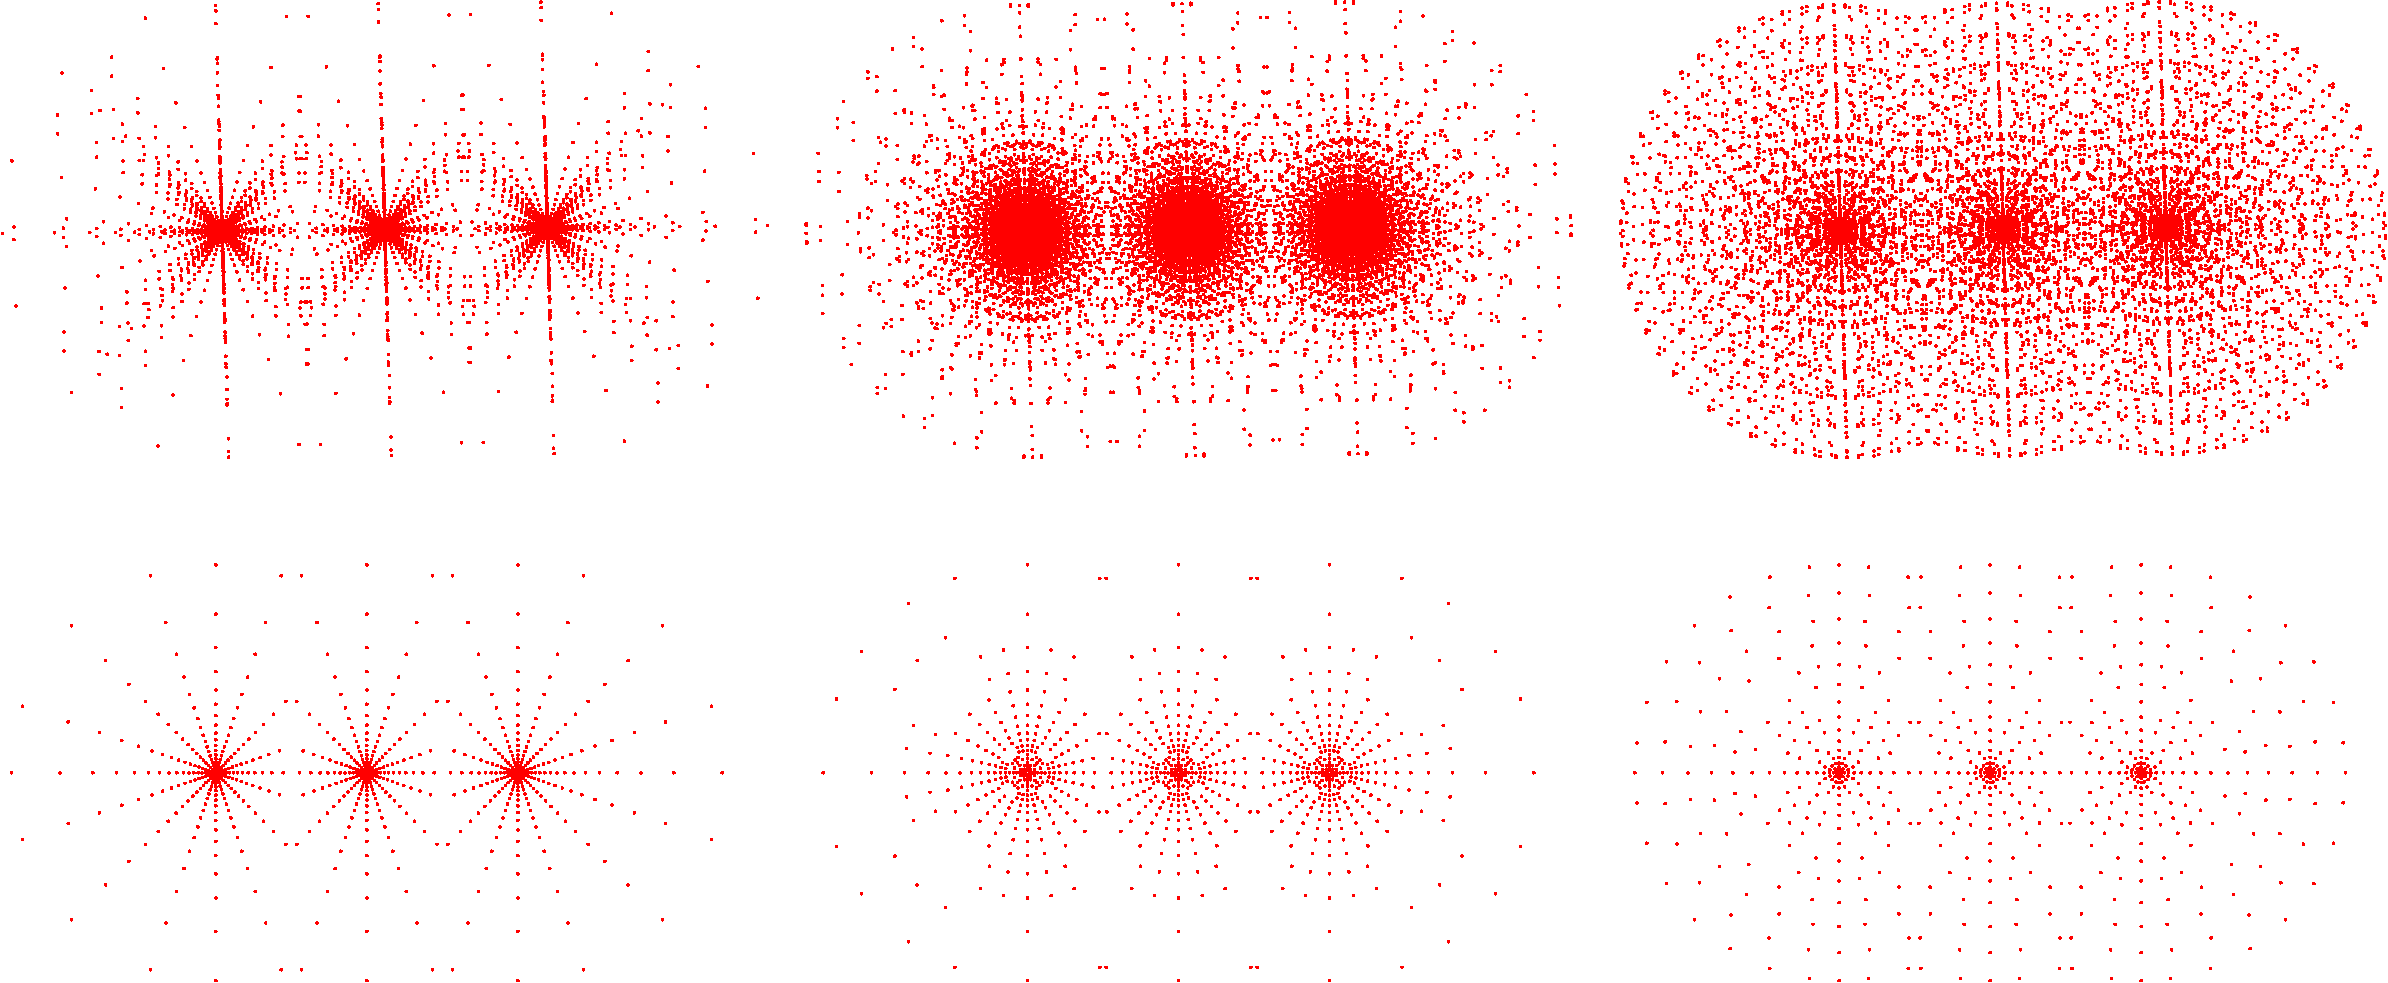
\includegraphics[width=\textwidth]{Figures/CO2_grid}
   \caption{Examples of point-distributions for a CO$_2$-molecules with $r_\text{max}=3\,$a.u. and $18$ spheres, in the upper row the full mesh, below cuts through the molecular plane.
   left: constant number of points, radial scheme (\ref{eq:son_map}) with $l=0.7$; centre: radial scheme (\ref{eq:son_map}) with number of points according to (\ref{eq:son_num}) with $l=0.7$; right: radial distribution (\ref{eq:tm_map}) with $l=0.7$, $p=2$ and number of points per sphere (\ref{eq:tm_num})}
   \label{fig:molmesh}
\end{figure}

Since in finite element theory the sphere neither needs to be really round nor is there any global functional defined on it,
the complicated distributions described above may be not even needed. 
An other approach therefore is to use an algorithm that gives just a more or less uniform distribution.

%Some explanations are given here:\\ %https://www.maths.unsw.edu.au/about/distributing-points-sphere
%Approach used for climate models: so-called geodesic grids: subdivision of polyhedra, projected onto the sphere\cite{geodesic1, geodesic2}, see also
%http://kiwi.atmos.colostate.edu/BUGS/geodesic/
%http://kiwi.atmos.colostate.edu/BUGS/pdf/ZM-grid.pdf
%http://kiwi.atmos.colostate.edu/BUGS/pdf/conservation.pdf
%http://kiwi.atmos.colostate.edu/BUGS/pdf/ccsr.pdf

The above mentioned techniques show the large variety of different approaches and it is not very clear which one will meet our needs best.
Moreover, here the problem is not only two dimensional but the whole sphere (not only its surface) needs to be subdivided. 
Hence, besides the question of a radial density of different spherical surfaces, also the number of points per sphere as function of the radial distance 
needs to be considered.

%Whether the approach of subdividing the atomic meshes into radial and angular parts as opposed to another volume tessellation can be questioned and may turn out to be inefficient.
%Application of Geodesic grid in calculating surface charges: \cite{geodes_charge}, also mentioning Connolly algorithm (refs 26, 29 therein).

%The second scheme has a divergence around $Nl=r_\text{max}$. 
%It can be shown that the condition $N\leq \frac rl $ is enough here to stabilise it.

%\textcolor{yellow}{
%If the above described procedures prove to be too inefficient, one could try to implement some WKB-based scheme similar to \cite{impLDVR} but in 3D.
%Thereby, the number of points in a given volume element is determined by $N_i=\frac{\alpha_i}{\alpha} N$ where $\alpha=\sum_i \alpha_i $ and
%\[ \alpha_i= \int_V dV \sqrt{2\mu (E-V(r))} \]
%.This ensures dense points there, where the potential is lowest and a coarse mesh far away; however, a consistent formulation in 3D would need to be invented.
%}
%
%To account for the molecular geometry and the general tendency of the photo electron to oscillate stronger in the vicinity of the nuclei, the mesh is built out of spheres, centred at the nuclear positions.
%Thereby, a study of Son \cite{Son_Chu0} had shown that it is numerically most efficient when the overlapping regions of these spheres are cut out.
%Figure \ref{fig:molmesh} shows an example for the water molecule.
%
%For the radial distribution we will use the the function
%\begin{equation}
%r_i = \frac{1+x_i}{1-x_i+\frac{2L}{r_{max}}} L \qquad x_i = \frac{2i}{N_r} -1
%\end{equation}
%suggested by Son \textit{et. al.}\cite{Son_Chu0, Son_Chu}.
%The parameters $N_r$, $L$ specifying the number of spheres and their distribution; the larger $L$ is, the denser are the spheres close to the centre.
%
%The optimal choice of these parameters as well as the angular distribution of points on the spheres is still an open question.
%Finally, after putting the points together as described above, they are connected to a Delaunay triangulation using \prog{tetgen} \cite{tetgen}. 
%Here additional points may be introduced to guarantee well-shaped elements (\texttt{i.e.} no sharp peaks).
%
%One scheme suggested by Son and Chu \cite{Son_Chu0}:
%\begin{equation} \label{eq:son_map}
%r_i=\frac{il}{N-i+\frac{lN}{r_\text{max}}} \qquad i=1,\hdots ,N 
%\end{equation}
%where $l$ is a parameter to chose.
%Own scheme:
%\begin{equation} \label{eq:tm_map}
%r_i=\frac{il}{\left( \frac Ni \right)^p \left(\frac{Nl}{r_\text{max}}-1\right) +1} \qquad i=1,\hdots ,N 
%\end{equation}
%where $l$ and $p\leq 1$ are parameters to chose. Thereby it is important to mention that in this scheme (in contrast to the above one) the (asymptotic for $r\rightarrow \infty$) maximum distance between two spheres is $l$ and hence could be physically chosen to $l\approx \frac \lambda 2$.
%
%The second scheme has a divergence around $Nl=r_\text{max}$. 
%It can be shown that the condition $N\leq \frac rl $ is enough here to stabilise it.

Besides the tricky question about this mapping, also the number of points per sphere depending on the radial distance needs to be considered. 
In \cite{Son_Chu0} this is chosen to be constant without further discussion but of course there are several possible design criteria as well.
Besides a constant number, also a constant spherical density (hence $N\propto r^2$) are possible; However, it might be sensible to follow a similar idea than in the radial mapping: Being fine close to the nuclei and get coarser with increasing distance.
In particular, I followed the design rule of keeping the space between points in radial direction similar to space between points in angular distribution.
Hence, $d_\text{spheric}=\sqrt{\frac{4\pi r_i^2}{N_i}}\approx r_i-r_{i-1}$.
For the above described radial schemes, this results in 
\begin{equation}\label{eq:tm_num}
N_i= \frac{4\pi}{ \left(1-\frac{i-1 }{i}\frac{N-i+\frac{lN}{r_\text{max}}}{N-i+1+\frac{lN}{r_\text{max}}}\right)^2 }
\end{equation}
for the first scheme and 
\begin{equation} \label{eq:son_num}
N_i= \frac{4\pi}{\left(1-\frac{i-1 }{i}\frac{ (\frac{N}{i})^p \left(\frac{lN}{r_\text{max}}-1\right)+1}{ (\frac{N}{i-1})^p\left( \frac{Nl}{r_\text{max}} -1 \right) +1 } \right)^2 }
\end{equation}
for the latter.

The respective radii and number of points per sphere are shown in Figure \ref{fig:maps}.\\
Special mapping schemes are the constant radial mapping $r_i=a i$ which corresponds to a constant spherical grid density $N_i=4\pi a^2 i^2$ and an exponential map $r_i=q^i r_0$ which would require a constant number of spherical grid points $N_i=\frac{4\pi q^2}{(1-q)^2}$ according to the rule derived above.

\begin{figure}
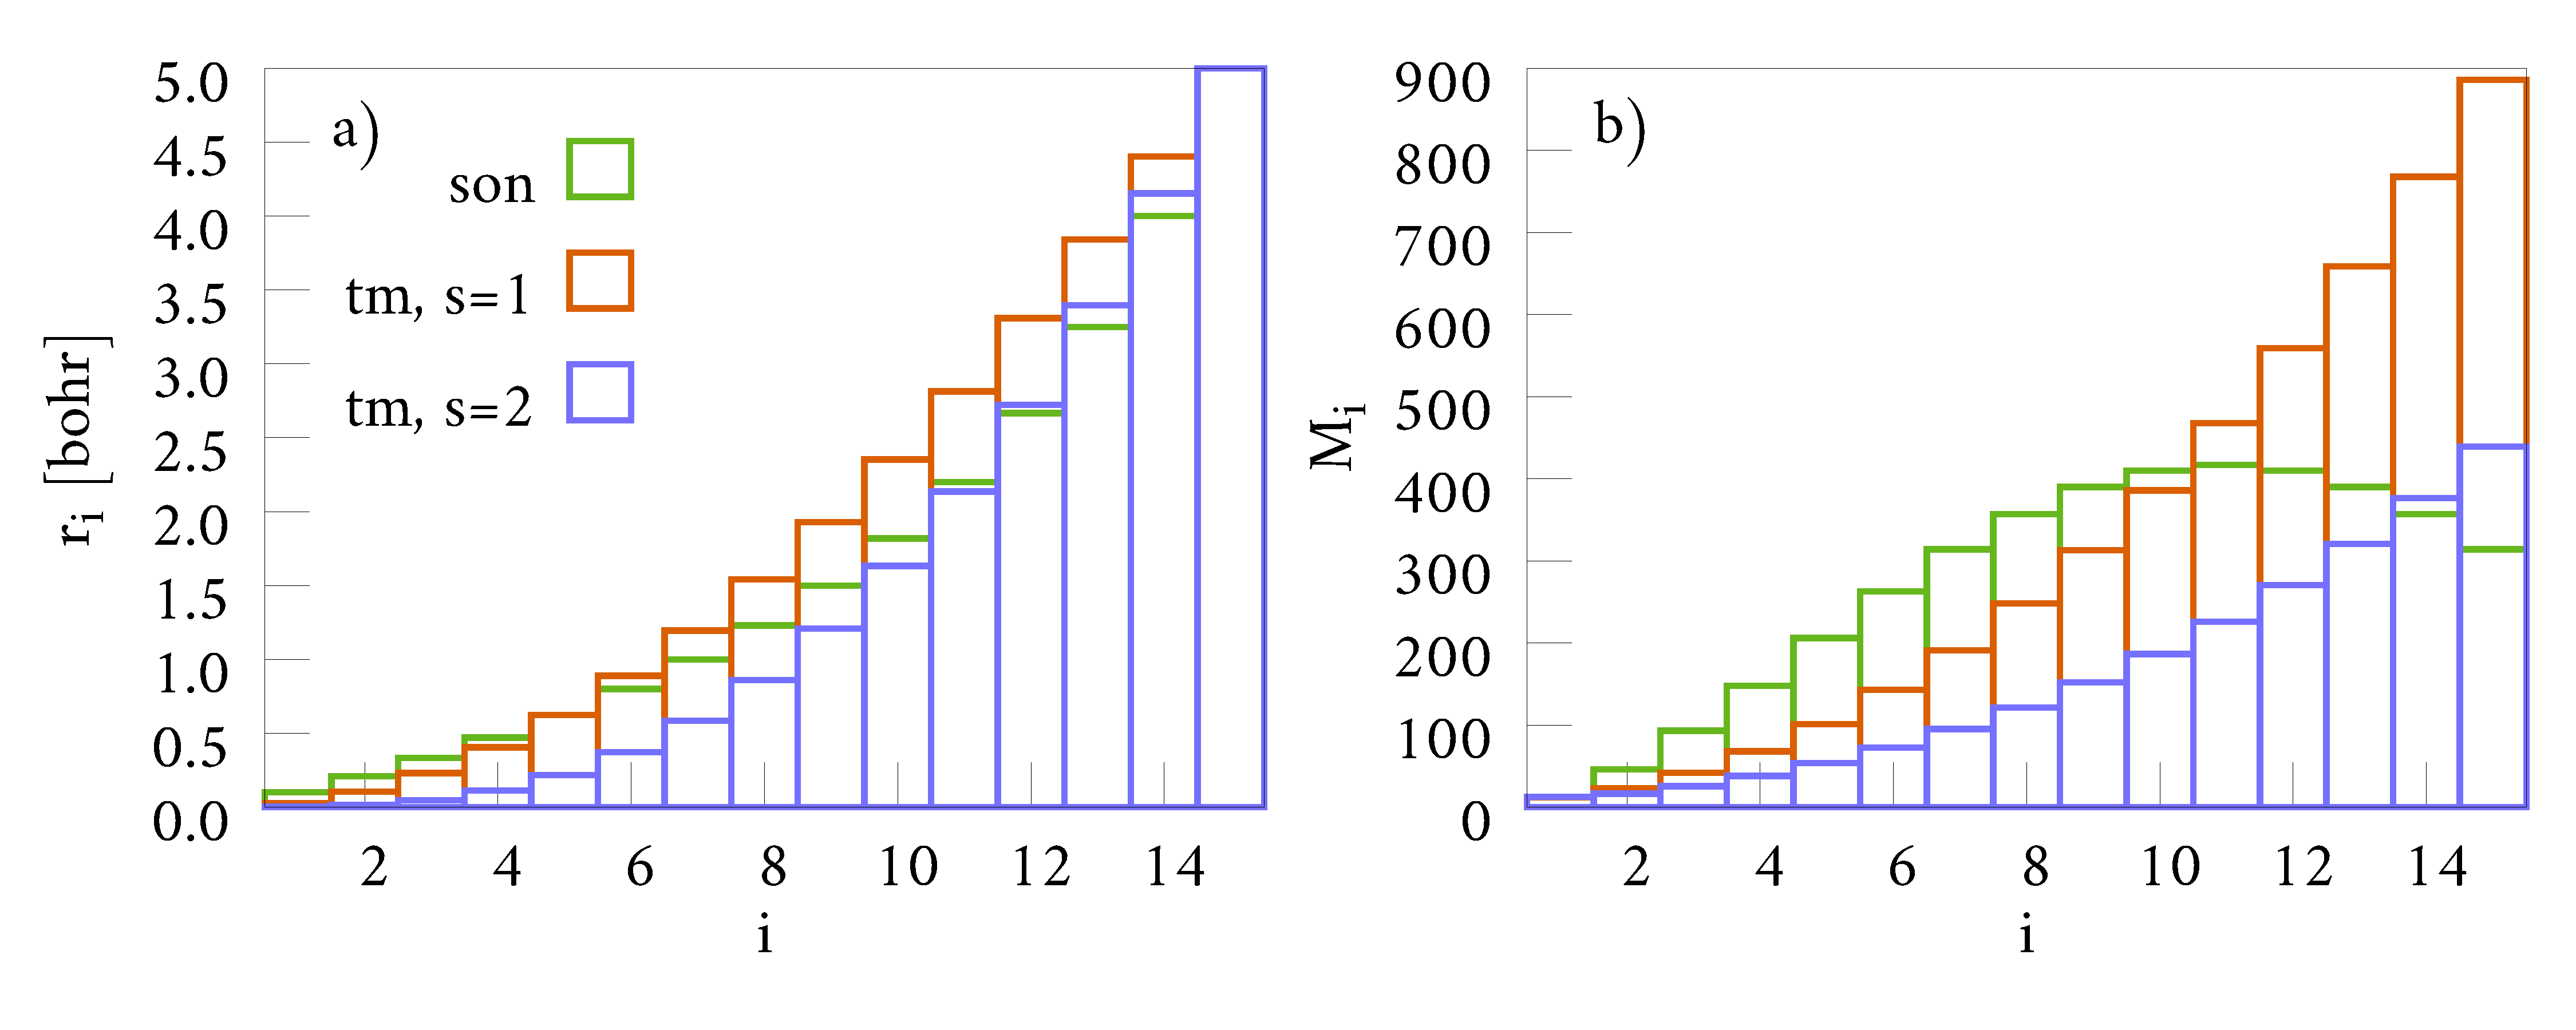
\includegraphics[width=\textwidth]{Data/radial_mapping}
\caption{Comparison of the radius (left) and number of points (right) of the different spheres ($N=15$, $r_\text{max}=5$ and $l=2$) for the different radial schemes (\ref{eq:son_map}) and (\ref{eq:tm_map}).}
\label{fig:maps}
\end{figure}

Since some of the spherical schemes described above allow only for certain numbers of points each, here, the best approximation is used respectively.
